\documentclass[12pt,letterpaper]{article}


\newcommand{\studentname}{Ben Bassett}

\title{\textsc{Lab 07: The RLC Circuit}}
\newcommand{\shorttitle}{The RLC Circuit}

\newcommand{\course}{PHY310}
\newcommand{\labdate}{10-22-2024}

%------------------------------------------------------------------------------------------------------------

\usepackage[letterpaper,left=1in,right=1in,bottom=1in,top=1in]{geometry}
\usepackage{fancyhdr}
\usepackage{subfigure}
\usepackage{graphicx}
\usepackage{amsmath}
\usepackage{cleveref}
\usepackage{booktabs}
\usepackage[british]{babel}
\usepackage[square,comma,numbers,sort&compress]{natbib}
\usepackage{csvsimple}
\usepackage{graphicx}
\usepackage{pgfplotstable}
\usepackage{textcomp,gensymb}
\usepackage{array}
\usepackage{tabu}
\usepackage{multirow}
\usepackage{url}
\usepackage{lipsum}
\usepackage{dsfont}
\pgfplotsset{compat=1.9}% supress warning
\begin{document}

%------------------------------------------------------------------------------------------------------------

\setlength{\parindent}{1em}
\setlength{\parskip}{0.5em}
\author{\course~Lab Journal \\ \\ \studentname} % \,\& \labpartner}
\date{\labdate}

\renewcommand\abstractname{Summary}

\pagestyle{fancy}
\fancyhead{}
\fancyhead[l]{\course:~\shorttitle}
\fancyhead[r]{\studentname}
\fancyfoot{}
\fancyfoot[C]{\thepage}
\renewcommand{\headrulewidth}{0pt}
\renewcommand{\footrulewidth}{0pt}

\renewcommand\bibname{References}

%------------------------------------------------------------------------------------------------------------

\renewcommand\abstractname{Abstract}
\maketitle

% COMMENT IN IF ASKED TO SUBMIT REPORT WITH ABSTRACT
%\begin{abstract}
%Maximum 200 words.
%\end{abstract}

\section{Purpose}
This lab aimed to measure the self-inductance of the Helmholtz coils using an RLC circuit.

\section{Experimental Apparatus}

Materials given were a Helmholtz coil, variable resistor, variable capacitor, voltmeter, function generator, multimeter, and various cables. My general setup is illustrated in Figure \ref{fig:setup}.

\begin{figure}[h]
    \centering
    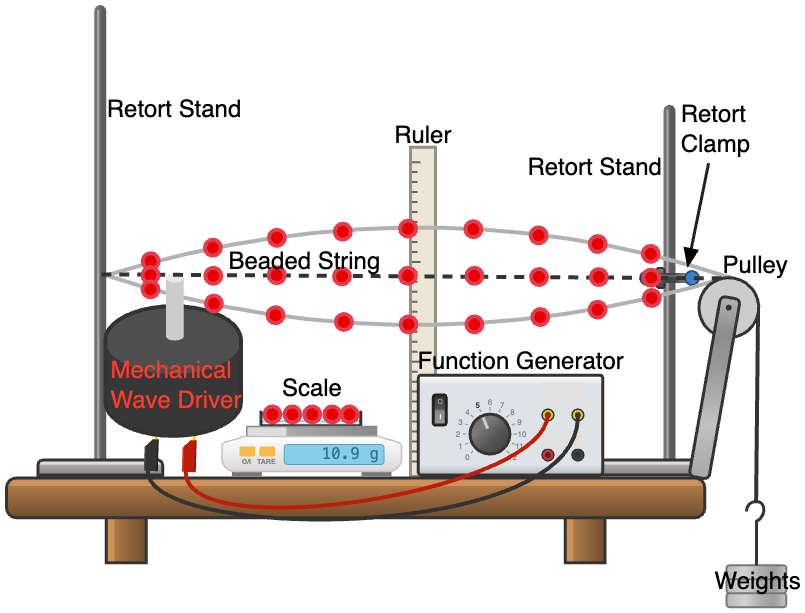
\includegraphics[width=6in]{images/setup.png}
    \caption{A diagram of my experimental setup}
    \label{fig:setup}
\end{figure}

% \pagebreak
\section{Procedure}

To begin, we connected the Helmholtz coil in series with a 50 $Ohm$ resistor and a 4 $\mu $F capacitor at either end of a function generator. We measured the actual attributes of the capacitor, resistor, and coil using multimeters.

We were told to assume for theoretical purposes a self-inductance of 0.02 Henries, so we computed the theoretical resonant frequency of the circuit with that value, as well as what we measured for the resistance and capacitance of the circuit.

Then we placed the voltmeter across the resistor and used the function generator at 4 Volts with a sinusoidal wave to sweep around our theoretical value to discover the actual self-inductance.

\section{Results}

We start with the series RLC circuit driven by an AC voltage source $V(t) = V_{0} \sin(\omega t)$, where $\omega = 2 \pi f$ is the angular frequency. The equation we use to model this (the current $I(t)$ through the circuit) is remarkably similar to our derivation for a driven damped harmonic oscillator!

\begin{equation}
L \frac{d^2 Q}{dt^2} + R \frac{dQ}{dt} + \frac{Q}{C} = V_{\text{source}}(t)
\end{equation}

Here, $Q$ is the charge, and $I(t) = \frac{dQ}{dt}$ is the current. We use an Ansatz for $I(t)$ of the form

\begin{equation}
I(t) = I_{0}\sin(\omega t - \phi)
\end{equation}

where $\phi$ is the phase shift between the current and the source voltage. As we saw in the lecture, the amplitude of the current $I_{0}$ can be found from the amplitude of the driving voltage $V_{0}$ and the properties of an RLC circuit:

\begin{equation}
I_{0} = \frac{V_{0}}{\sqrt{R^2 + \left( \omega L - \frac{1}{\omega C} \right)^2}}
\end{equation}

Since we want RMS voltage, we remember from painful homework integrals that the RMS value of a sinusoidal function $A \sin(\omega t)$ is $\frac{A}{\sqrt{2}}$, so the RMS voltage across the resistor is:

\begin{equation}
V_{\text{Resistor RMS}} = \frac{I_{\text{peak}} R}{\sqrt{2}}
\end{equation}

Therefore

\begin{equation}
V_{\text{Resistor RMS}} = \frac{V_{0} R}{\sqrt{2} \sqrt{R^2 + \left( \omega L - \frac{1}{\omega C} \right)^2}}
\label{eqn:fit}
\end{equation}

Now we have an expression for our RMS voltage across the resistor as a function of frequency $\omega$, resistance $R$, capacitance $C$, and the inductance $L$ which we want to know.

See Table \ref{tab:voltage_measurements} of $V_{\text{Resistor RMS}}$ with respect to voltage. Errors have been propagated.

\begin{table}[h]
\centering
\begin{tabular}{|c|c|c|}
\hline
Frequency (Hz) & RMS Voltage (V) & Voltage Amplitude (V) \\
\hline
420.00 & 2.7310 $\pm$ 0.0273 & 3.8622 $\pm$ 0.0386 \\
430.00 & 2.8046 $\pm$ 0.0280 & 3.9664 $\pm$ 0.0397 \\
440.00 & 2.8792 $\pm$ 0.0288 & 4.0719 $\pm$ 0.0407 \\
450.00 & 2.9462 $\pm$ 0.0295 & 4.1665 $\pm$ 0.0417 \\
460.00 & 3.0069 $\pm$ 0.0301 & 4.2524 $\pm$ 0.0425 \\
470.00 & 3.0611 $\pm$ 0.0306 & 4.3291 $\pm$ 0.0433 \\
480.00 & 3.1075 $\pm$ 0.0311 & 4.3947 $\pm$ 0.0439 \\
490.00 & 3.1476 $\pm$ 0.0315 & 4.4514 $\pm$ 0.0445 \\
500.00 & 3.1779 $\pm$ 0.0318 & 4.4942 $\pm$ 0.0449 \\
510.00 & 3.1986 $\pm$ 0.0320 & 4.5236 $\pm$ 0.0452 \\
520.00 & 3.2109 $\pm$ 0.0321 & 4.5410 $\pm$ 0.0454 \\
530.00 & 3.2161 $\pm$ 0.0322 & 4.5483 $\pm$ 0.0455 \\
540.00 & 3.2064 $\pm$ 0.0321 & 4.5345 $\pm$ 0.0453 \\
550.00 & 3.2034 $\pm$ 0.0320 & 4.5304 $\pm$ 0.0453 \\
560.00 & 3.1833 $\pm$ 0.0318 & 4.5018 $\pm$ 0.0450 \\
570.00 & 3.1548 $\pm$ 0.0315 & 4.4615 $\pm$ 0.0446 \\
580.00 & 3.1213 $\pm$ 0.0312 & 4.4142 $\pm$ 0.0441 \\
590.00 & 3.0947 $\pm$ 0.0309 & 4.3765 $\pm$ 0.0438 \\
600.00 & 3.0516 $\pm$ 0.0305 & 4.3156 $\pm$ 0.0432 \\
610.00 & 3.0156 $\pm$ 0.0302 & 4.2647 $\pm$ 0.0426 \\
\hline
\end{tabular}
\caption{RMS Voltages and Amplitudes at Frequencies}
\label{tab:voltage_measurements}
\end{table}

To compute a theoretical value to base our experimental results around, I used Wolfram Alpha to take the derivative of $\sqrt{\left(\frac{1}{LC}- \omega^2\right)^2+\left(\frac{R\omega}{L}\right)^2}$ and set it equal to zero. We used our capacitance and resistance, and a theoretical value of 0.02 Henries for self-inductance, and found the theoretical resonant frequency of that expression to be 468 Hz.

To find the actual self-inductance, I used Equation \ref{eqn:fit} to fit our data, shown in Figure \ref{fig:fit}. Scipy does all the heavy lifting for us, and we're left with the conclusion that the real resonant frequency was $\mathbf{530}\textbf{ Hz}$, and $L= \mathbf{0.0209 \pm 0.0054} \textbf{ Henries}$.

\begin{figure}[ht]
    \centering
    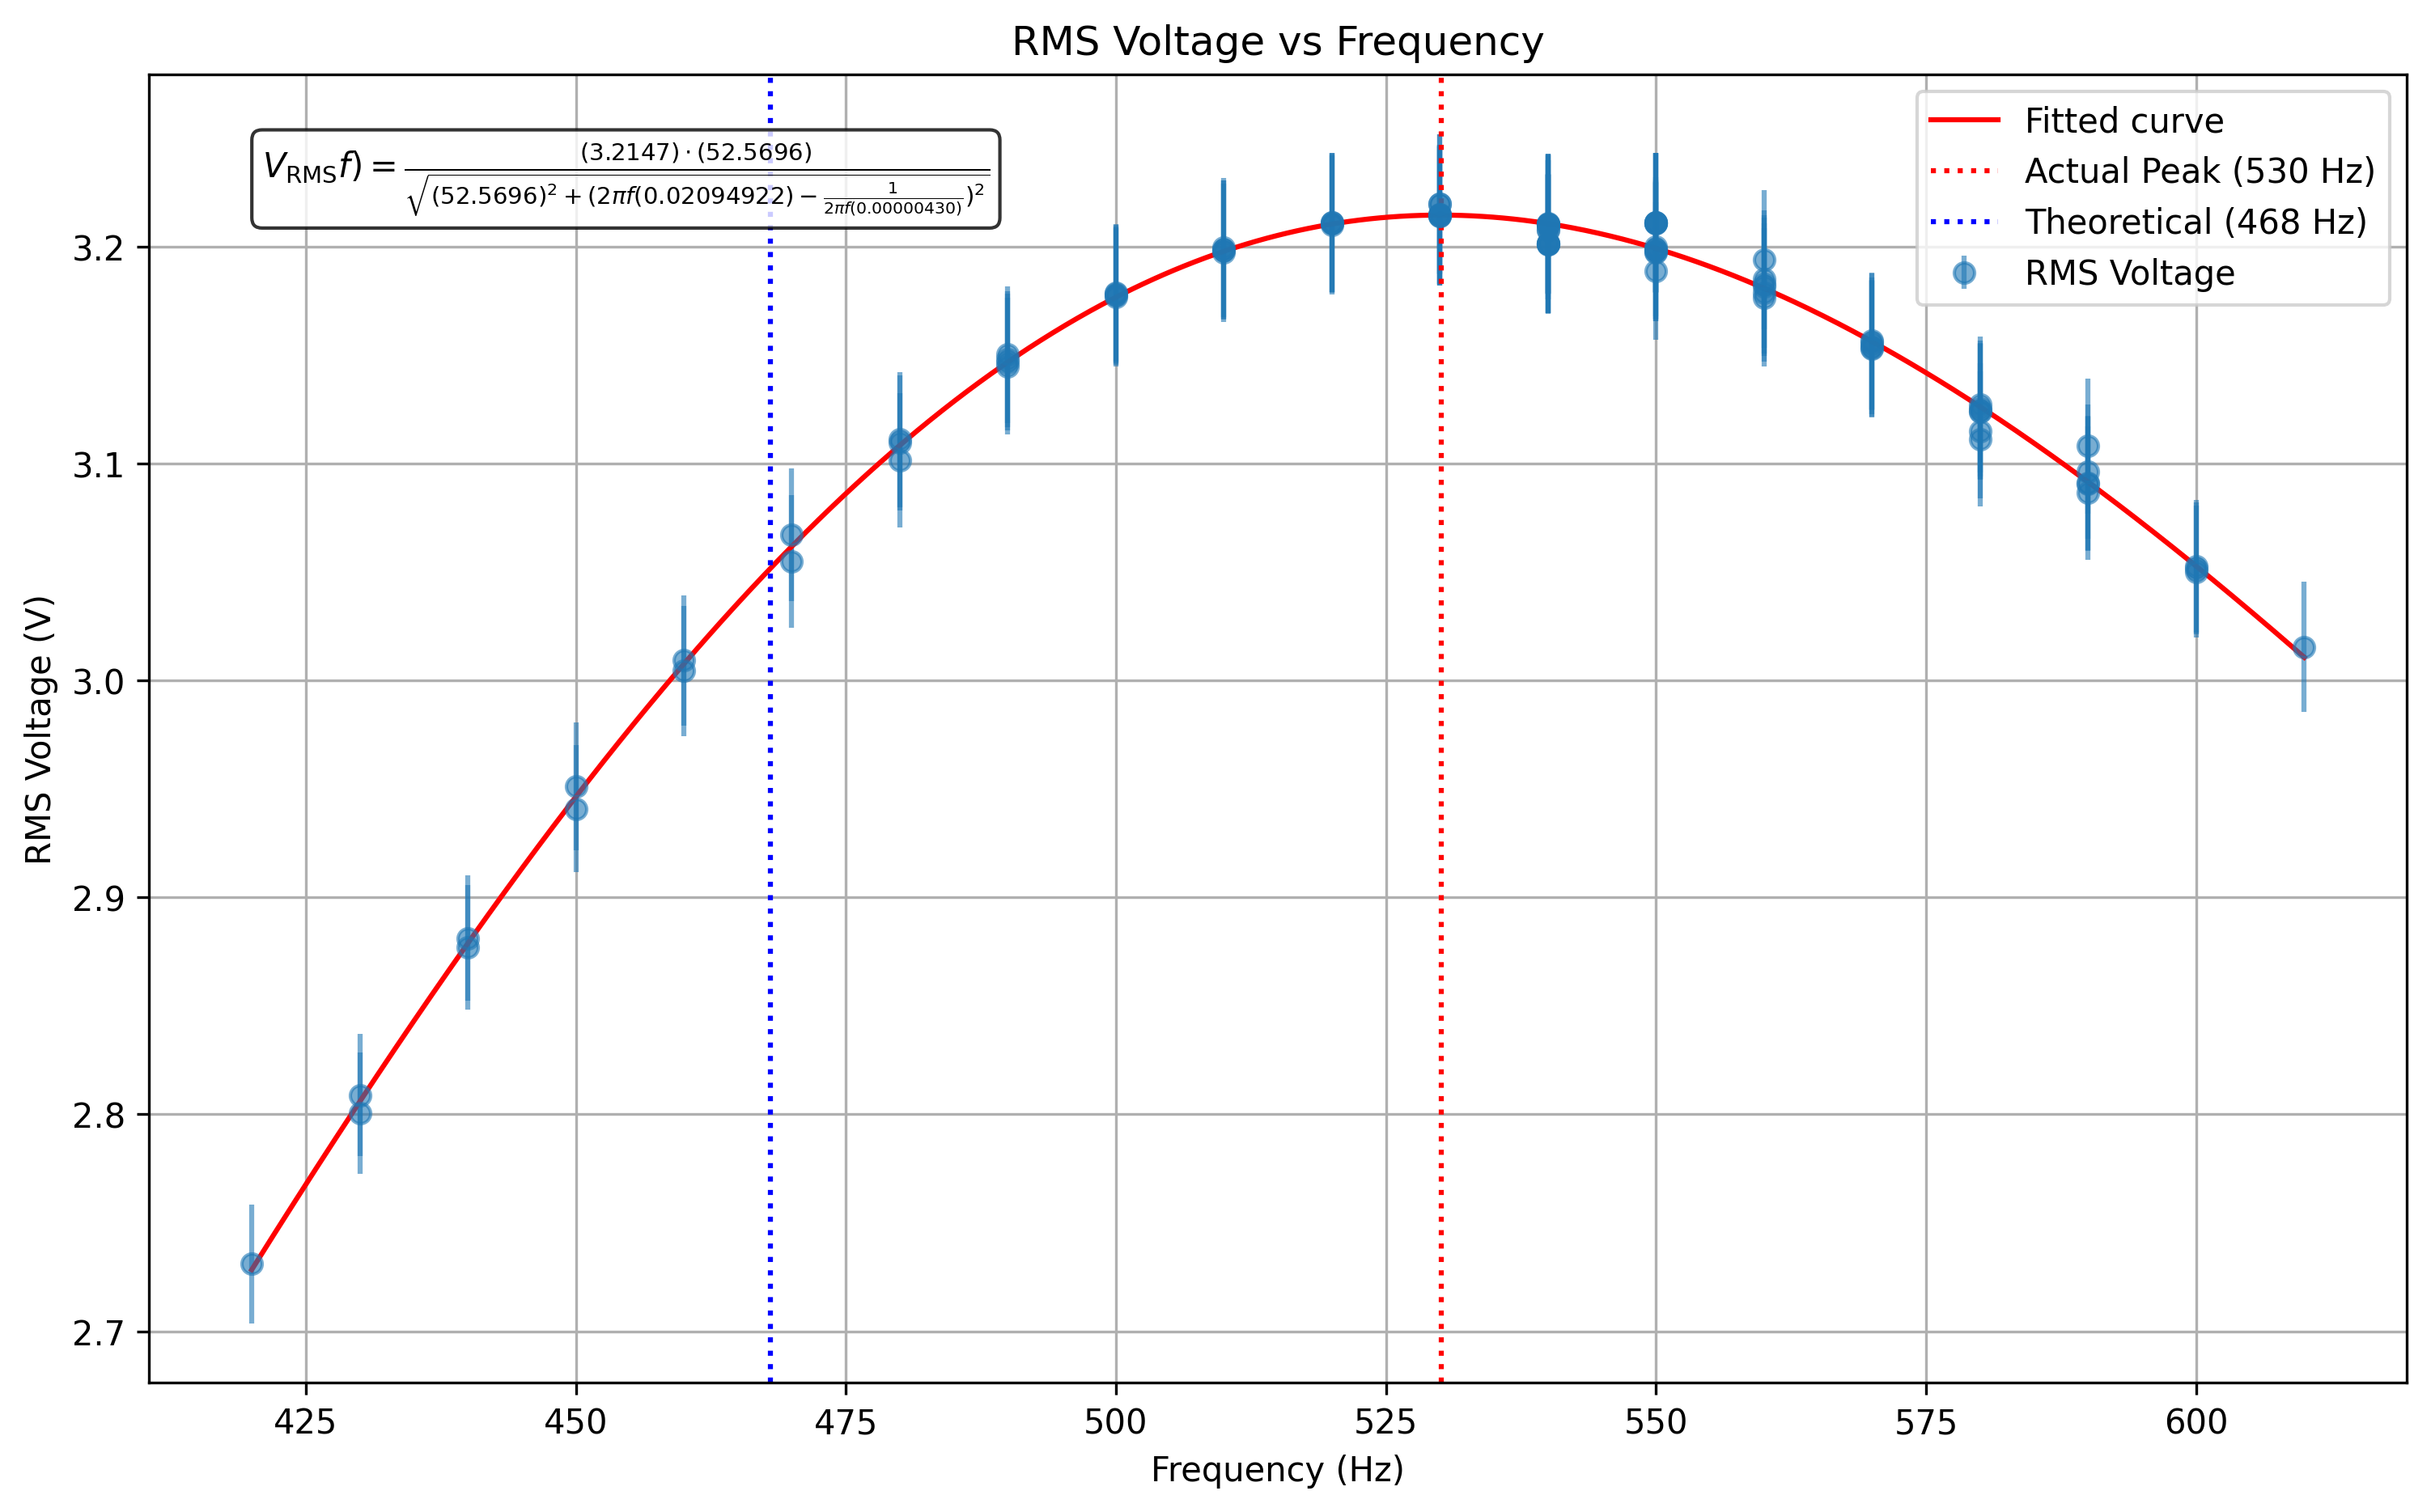
\includegraphics[width=6.5in]{images/voltage_amplitude_vs_frequency_fitted.png}
    \caption{Voltage plotted against amplitude}
    \label{fig:fit}
\end{figure}


\section{Conclusions}

Comparing this result to the results from Lab 6, my inductance there was measured to be $\mathbf{0.0393 \pm 0.0004}\textbf{ Henries}$ where here it was $\mathbf{0.0209 \pm 0.005} \textbf{ Henries}$. This makes me think that something in one of the labs was off by a factor of two. Not bad, all things considered. Our samples showed a clear resonant frequency, which lead to a good, not highly error-prone computation for the self-inductance.


% \bibliographystyle{unsrtnat}
% \bibliography{references}

\end{document}
